\chapter{Система имитационного моделирования.}

\section{Архитектура подсистемы имитационного моделирования}

В данном разделе будут рассмотрено внутренние устройство элемента архитектуры ПО (\ref{ris:arh1}), отвечающего за имитационное моделирование. 
Работа имитацонной модели состоит из следующих этапов:

\begin{enumerate}
    \item Создание шаблона продуктов. Шаблон представляет из себя структуру данных, являющийся отображением технологической карты одной единицы продукции.
	\item Создание заказа. Заказ представляет из себя список структур данных, включающим в себя шаблон продукта и необходимое количество.
	\item Следующим этапом является развертывание единого плана на основе заказа. Производсвенный план описывает совокупность операций\footnote{Так как технологическая карта описывается набором операций, а заказ описывается перечнем технологических карт и их количеством, появилась возможность описать план совокупностью операций.} и состояние ресурсов.
    \item Пошаговая реализация плана с учетом ресурсных ограничений, где каждый раз при расчете операции обновляется информации о состоянии ресурсов.
\end{enumerate}

Работа имитационного моделирования представлена на рисунке \ref{ris:alg}
\begin{figure}[H]
    \center{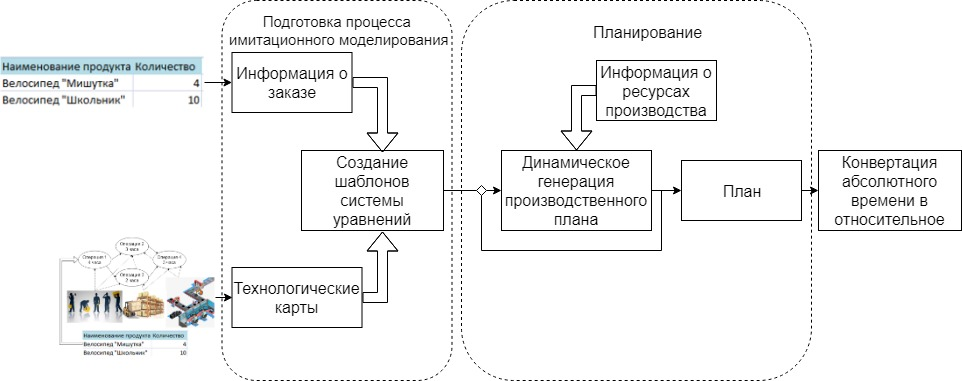
\includegraphics[width=1\linewidth]{fig/alg.jpg}}
    \caption{Визаулизация работы имитацонного моделирования}
    \label{ris:alg}
\end{figure}

\section{Входные и выходные данные}

\subsection{Входные данные}
В данном разделе приведены входные данные для имитационной модели. Благодаря модульности данного элемента ПО, в перечень включены данные не учтенные в текущей реализации, добавление данных планируется в будущем. Эти данные \textit{помечены курсивом}.

\begin{itemize}
	\item ЦПВ - цеховая последовательность выпуска (выпуск продукции осуществляется в порядке, в котором они записаны в ЦПВ):
		\begin{itemize}
			\item наименование продукции;
			\item количество единиц продукции;	
			\item технологическая карта.
		\end{itemize}			
	\item Технологические карты, подробнее смотри (\ref{assembly_line_balancing:input_data}).
	\item Производственные ресурсы;
	\item \textit{Трафик доступности ресурсов};
	\item \textit{Структура цеха};
	\item \textit{Минимальное время участия ресурса в операции};
	\item \textit{Штрафы за переключение ресурса с одной операции на другую}. 
\end{itemize}

\subsection{Выходные данные}

\begin{itemize}
	\item Расчетные данные:	
		\begin{itemize}
			\item Перечень всех операций для всех единиц продукции ЦПВ;
			\item Время начала всех операций;
			\item Время окончания всех операций;
			\item \textit{Производственные ресурсы, привлекаемые к выполнению операции};
			\item \textit{Время начала и конца участия ресурса в операции};
			\item \textit{Загрузка производственных ресурсов}.
		\end{itemize}		
	\item Визуализиация данных пользователю:
		\begin{itemize}
			\item Расписания для производственных ресурсов;
			\item Диаграммы Ганта выпуска разных видов продукции;
			\item Визуализация загрузки производственных ресурсов.
		\end{itemize}		 
\end{itemize}

\section{Этапы имитационного моделирования}
В данном разделе подробно описаны все этапы имитационного моделирования.
На изображении (\ref{ris:DataFlow}) приведена диаграмма потоков данных.

\begin{figure}[H]
    \center{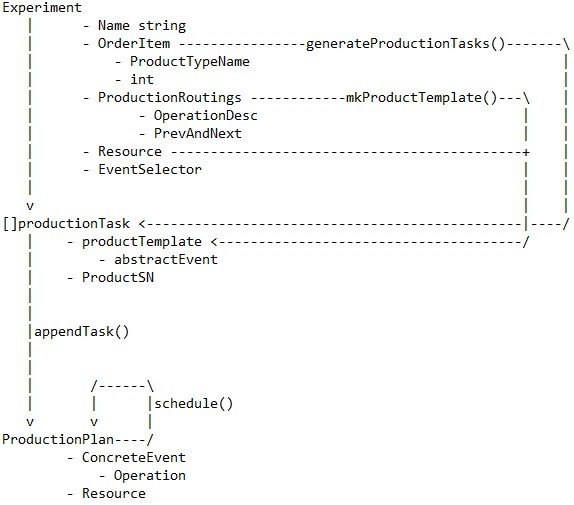
\includegraphics[width=1\linewidth]{fig/MkExperimentDataFLow.jpg}}
    \caption{Data flow imcore}
    \label{ris:DataFlow}
\end{figure}

\subsection{Предобработка технологических карт}

\subsubsection{Входные данные}
Входными данными для данного элемента ПО является технологическая карта с конфигурациями ресурсов\footnote{Примером конфигурации ресурса может являться вычисление длительности операции на основе количества персонала, привязанного к операции.}. 

\subsubsection{Выходные данные}
Выходными данными являются технологическая карта с зафиксированными значениями.

\subsubsection{Процесс предобработки}
Одним из первых этапов работы алгоритма имитационного моделирования является подготовка входных данных, полученных из базы данных. 

На текущий момент реализована небольшая часть функционала отвечающую за предварительную обработку. Одной из таких функций является расчет длительности операций. Так как длительность операций является переменной величиной, зависимой от трудоемкости и количества людей выполняющих операцию, существует 4 настройки ресурса:

\begin{enumerate}
    \item Минимальная, при этом на операцию назначается минимальное количество людей, отсюда и длительность операции становится максимальной;
    \item Максимальная, при этом на операцию назначается максимальное количество людей, отсюда и длительность операции становится минимальной;
    \item Средняя при этом на операцию назначается среднее количество людей, отсюда и длительность операции становится средней;
    \item Случайная, при этом количество персонала на операцию выбирается случайным образом. 
\end{enumerate}

Также одной из возможностей предварительной настройки является алгоритм выбора оперции\footnote{В тех случаях, когда на этапе планирования есть независимые операции}. На данный момент существует 2 конфигурации:

\begin{itemize}
    \item стандартная, при которой выбор осуществляется строго по порядку расположения в структурах данных
    \item случайная, при этом случайным образом выбирается одна из возможных операций, которые доступны в данный момент 
\end{itemize}

Возможность менять входные данные являются важным этапом обработки входных данных полученных из базы данных, позволяя при этом подготовить данные для дальнейшей обработки, а также гибко менять параметризуемые величины, чем и достигается большая вариативность необходимая для поиска оптимального значения. 

\subsection{Создание шаблона продукта}

\subsubsection{Входные данные}
Входными данными для данного элемента имитационной модели является технологическая карта с фиксированными значения (прошедшая обработку после базы данных).

\subsubsection{Выходные данные}
\label{imcore:mkProductTemplate_output_data}
Выходными данными являются структура данных, включающая в себя набор событий и привязок ресурсов к каждому событию.

\subsubsection{Описание реализации}
Для начала необходимо определить для чего нужны события. Как говорилось ранее любая технологическая карта состоит из перечня операций. В процессе работы было принято решение разделить операцию на события. Операция определяется двумя событиями: началом и концом. Такое разделение не случайно и вызвано необходимостью раздельной работы с началом и концом операций. Примером, когда это необходимо, является занятие и освобождение ресурса предприятия. При начальном событии алгоритм учитывает, то что данная операция потребляет ресурсы, при этом основным индикатором является начальное состояние. При конченом событии, когда ресурсы на операции использованы, происходит процесс высвобождения ресурсов, состояние ресурсов обновляется.

Основной задачей процесса создания шаблона продукта является подготовка необходимых структур данных для дальнейшей работы имитационной модели. На диаграмме потоков данных (\ref{ris:DataFlow}) данный процесс именуется, как - mkProductTemplate(). В результате работы, mkProductTemplate() создает шаблон продукта необходимый для структуры описывающий заказ.

\subsection{Создание заказа}

\subsubsection{Входные данные}
Входными данными является перечень продуктов и количество каждого продукта из этого перечня.

\label{imcore:generateProductionTasks_output_data}

\subsubsection{Выходные данные}
Выходными данными является список структур описываемых в разделе \ref{imcore:mkProductTemplate_output_data}, то есть шаблон и количество данного продукта.

\subsubsection{Описание реализации}
На диаграмме потоков данных \ref{ris:DataFlow} процесс создания заказа называется - generateProductionTasks(). Основной задачей функции заказа является генерация шаблонов продуктов в зависимости от их количества, при этом каждый однотипный шаблон имеет уникальный идетификатор (серийный номер).


\subsection{Планирование}

\subsubsection{Входные данные}
Входными данными для функции планирования является производственное задание на одну единицу продукции, полученное из списка сформировавшемся на этапе создания заказа (\ref{imcore:generateProductionTasks_output_data}).

\subsubsection{Выходные данные}
Выходными данными является производсвенный план, состоящий из событий, операций и состояния ресурсов.

\subsubsection{Описание реализации}
На данном этапе из списка полученного на предыдущем этапе формирования заказа, берется 

\subsection{Алгоритм модели Staff}

\subsection{Оптимизация на уровне имитационного моделирования}

\subsubsection{Метод полного перебора}
Примером оптимизации может служить случайный выбор следующей операции при планировании, данный выбор возможен только в случаях одновременного выполнения нескольких независимых операций. Таким образом достигается вариативность при котором из разных реализаций, выбирается наилучший вариант. На рисунке (\ref{ris:Force}) изображены технологическая карта продукта и два плана, который были построены в результате случайного выбора операций.

\begin{figure}[H]
    \center{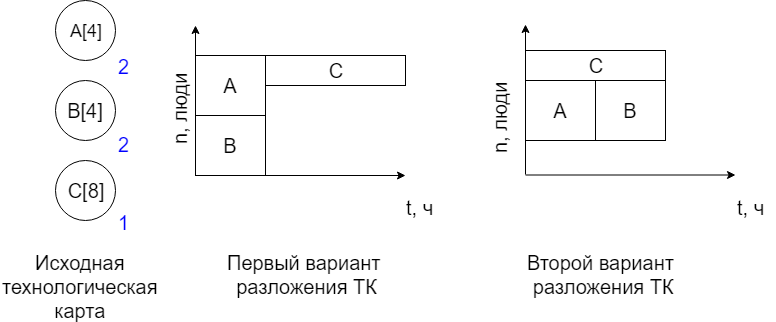
\includegraphics[width=1\linewidth]{fig/DecompositionOfTk.png}}
    \caption{Два плана, полученные путем перебора исходной технологической карты}
    \label{ris:Force}
\end{figure}

\subsubsection{Методы оптимизации полного перебора}

\section{Результаты работы имитационной модели}